\documentclass[runningheads]{llncs}
\usepackage[T1]{fontenc}
\usepackage{graphicx}
\usepackage{booktabs}
\usepackage{amsmath}
\usepackage{amssymb}
\usepackage{tikz}
\usetikzlibrary{positioning,arrows.meta,fit}
\graphicspath{{figures/}}

\begin{document}

\title{Automated Skin Disease Detection from Dermoscopic Images with Explainability Analysis}
\titlerunning{Automated Skin Disease Detection with Explainability Analysis}

\author{Tashmika Pillay \and Serestina Viriri}
\authorrunning{T. Pillay and S. Viriri}
\institute{Discipline of Computer Science, University of KwaZulu-Natal\\
\email{223097300@stu.ukzn.ac.za, viriris@ukzn.ac.za}}

\maketitle

\begin{abstract}
Deep learning models for dermoscopic images are often reported with a single training run, a single headline metric and heatmaps that are shown but never tested. This paper studies a compact hybrid model that joins a MobileNetV3-Small backbone to a four layer Transformer encoder, and asks which of its design choices actually matter on the HAM10000 dataset. All experiments use a split by lesion, and the comparison models are trained under one identical pipeline with three random seeds. At an input size of 448 pixels the hybrid reaches an accuracy of 0.821, a balanced accuracy of 0.729, a macro F1 of 0.699 and a macro AUROC of 0.946 with 8.3 million parameters. Under an equal budget at 224 pixels, EfficientNet-B3 is the strongest model, while the hybrid is close to ViT-B/16 at about one tenth of its size, ahead on balanced accuracy and behind on accuracy and macro F1. The ablation shows that ImageNet pretraining matters most, that correcting for class imbalance twice hurts the model, and that aggressive hair removal lowers its scores. Removing the Transformer changes little and leaves a model of 1.15 million parameters with similar results. Grad-CAM and attention maps are evaluated with deletion and insertion curves against a centre prior, and they outperform it on insertion but not on deletion. Calibration, clinical error rates and a CLIP based input check are also reported. The results show where a lightweight hybrid stands and what its explanations can and cannot show.

\keywords{Skin lesion classification \and Dermoscopy \and Hybrid CNN Transformer \and Ablation study \and Explainable AI}
\end{abstract}

\section{Introduction}

Skin diseases are among the most common health problems worldwide \cite{hay2014}, and melanoma in particular is far easier to treat when it is found early. Dermoscopy improves diagnostic accuracy over examination with the naked eye \cite{vestergaard2008}, but it depends on trained specialists who are not available in every clinic. Automated classification of dermoscopic images has therefore attracted sustained interest since deep convolutional networks were shown to match dermatologists on selected tasks \cite{esteva2017}.

Two families of models dominate this work. Convolutional neural networks (CNNs) such as EfficientNet \cite{tan2019} extract local texture and colour patterns efficiently. Vision Transformers \cite{dosovitskiy2021} relate distant image regions through self attention \cite{vaswani2017} but usually need more data and more computation. Hybrid designs pass CNN features to a Transformer in the hope of getting both local detail and global context \cite{chen2021}. For a deployment setting with modest hardware, a small hybrid is an attractive idea.

Three weaknesses recur in the literature and make such claims hard to judge. First, HAM10000 \cite{tschandl2018} is heavily imbalanced, with two thirds of its images in one class, so a model can score well on some metrics while doing worse than a trivial rule on others. Second, many comparisons rest on a single training run, which cannot separate a real difference from run to run variation. Third, explanations are commonly presented as a handful of heatmaps, although saliency maps can look convincing without reflecting what a model has learned \cite{adebayo2018}. Because the lesion sits near the centre of most dermoscopic images, a heatmap on the centre is in any case weak evidence that the model attends to anything meaningful.

This paper responds to those weaknesses with a study of one lightweight hybrid model. Its contributions are as follows.
\begin{enumerate}
\item A like for like comparison of the hybrid with EfficientNet-B3 and ViT-B/16, trained under one pipeline with three seeds and reported with confidence intervals.
\item An ablation that changes one design choice at a time, covering pretraining, class imbalance handling, hair removal, input resolution and the Transformer itself.
\item A conservative hair removal step, motivated by a measurement of how much of each image a standard approach alters.
\item A quantitative test of explanation faithfulness against a centre prior and a random baseline.
\item A clinical reading of the results, including calibration, per class error rates and the behaviour of a CLIP based input check.
\end{enumerate}
The outcome is mixed, and we report it as such. The hybrid is a sound classifier, but it does not beat EfficientNet-B3, and its Transformer accounts for most of its size without a matching gain in accuracy.

\section{Related Work}

Esteva et al.\ \cite{esteva2017} trained a CNN on 129,450 clinical images and matched dermatologists on two binary tasks. The result was influential, but the images were private and the tasks binary, so the work cannot be reproduced or extended to the multiclass problem studied here. Tschandl et al.\ \cite{tschandl2018} addressed the data problem by releasing HAM10000, a public set of 10,015 dermoscopic images in seven classes, which became the basis of the ISIC 2018 challenge. The dataset brings difficulties of its own: about two thirds of the images are nevi, and many lesions are photographed more than once. The challenge ranked entries by balanced accuracy, and the best submission reached 0.885 on the held out test set \cite{codella2019}. A ranking of this kind rewards a single score, so the size, cost and interpretability of the leading models were not part of the comparison, although these are the properties that matter when a model must run on modest hardware.

Later studies report higher figures. Haque et al.\ \cite{haque2026}, for example, report an accuracy of 91.15\% and a macro F1 of 85.45\% with an EfficientNetV2-L backbone, channel attention and progressive training. Results of this kind come from backbones far larger than a lightweight model, and they can only be compared fairly when the split is made over lesions, because a split made over images can place views of the same lesion in both the training and test sets and so inflate the score. Daneshjou et al.\ \cite{daneshjou2022} point to a weakness that affects the whole field: models trained on public dermatology data perform worse on darker skin tones, which are rare in those datasets.

The Vision Transformer \cite{dosovitskiy2021} relates all regions of an image through self attention \cite{vaswani2017}, but its authors found that it trails CNNs unless it is pretrained on very large datasets. This is a poor fit for medical imaging, where labelled data are limited. Hybrid models such as TransUNet \cite{chen2021} reduce the demand for data by feeding CNN features to a Transformer. TransUNet, however, was designed for segmentation with a large backbone, and hybrid classifiers are rarely compared with the same model with the Transformer removed, so it is seldom shown that the Transformer earns its cost. A similar question applies to pretraining. Transfer from ImageNet \cite{deng2009} is standard practice, yet Raghu et al.\ \cite{raghu2019} found that it brought little gain in performance on retinal and chest images and that small models performed comparably to large ones. Their study did not include dermoscopy, so whether pretraining matters for a compact skin lesion model remains open.

Preprocessing has received less critical attention than architecture. For hair, DullRazor \cite{lee1997} introduced the common recipe of a morphological filter that finds dark thin structures, followed by interpolation over them, and later work often fills the detected pixels with general inpainting methods such as that of Telea \cite{telea2004}. These methods were judged mainly on how cleanly the hair disappears, not on what they do to a classifier. A filter tuned to catch every hair also marks lesion borders, pigment network and skin texture, and repainting those regions can remove the very structures a classifier needs. The effect of hair removal on classification accuracy is rarely measured, and the step is usually applied with fixed settings.

Explanation methods raise a similar problem of evidence. Grad-CAM \cite{selvaraju2017} and SHAP \cite{lundberg2017} are the most widely used in this area, and they are usually reported as a few example heatmaps judged by eye. Adebayo et al.\ \cite{adebayo2018} showed why this is not enough: some saliency methods produce nearly the same map when the weights of the model are randomised, so a convincing picture is no proof that a map reflects the model. Lucieri et al.\ \cite{lucieri2022} proposed explanations expressed in dermatological concepts, which are closer to clinical reasoning, but this requires images labelled with those concepts, which HAM10000 does not provide. Whewell et al.\ \cite{whewell2026} review explainable methods for skin lesion classification, with attention to how the choice of dataset shapes the conclusions that can be drawn. Petsiuk et al.\ \cite{petsiuk2018} proposed deletion and insertion curves as a quantitative test of faithfulness, but the test was designed for natural images. In dermoscopy the lesion is almost always centred, so a map that simply highlights the middle of the image can score well without revealing anything about the model. A fair test therefore needs a centre baseline, which to our knowledge is rarely included.

Rare classes motivate a different line of work. Prototypical networks \cite{snell2017} classify from a few labelled examples per class, and CLIP \cite{radford2021} classifies from text descriptions without any task specific training. Both are attractive for rare skin conditions, but they were developed and evaluated on general images, and CLIP was trained on image and text pairs collected from the internet rather than on dermoscopy. How well either transfers to rare lesion types, and whether CLIP can at least recognise that an image shows a skin lesion, must be measured before either is relied on.

Taken together, earlier work leaves four gaps. Strong results on HAM10000 are usually reported for large models from a single training run, and differences in how the data are split make them hard to compare. Hybrid models are seldom tested with the Transformer removed or against standard models under the same pipeline. Preprocessing steps such as hair removal are applied without measuring their effect. Explanations are shown rather than tested, and rarely against the trivial explanation that the lesion is in the centre. This paper addresses each of these gaps in turn.

\section{Methods and Techniques}

\subsection{Dataset and Split}

We use HAM10000 \cite{tschandl2018}. The seven classes are melanocytic nevus (nv), melanoma (mel), benign keratosis (bkl), basal cell carcinoma (bcc), actinic keratosis and intraepithelial carcinoma (akiec), vascular lesion (vasc) and dermatofibroma (df). The 10,015 images come from 7,470 distinct lesions. We divide the lesions, not the images, into training, validation and test sets in the proportions 70, 15 and 15 percent with a fixed seed, so that no lesion contributes images to more than one set. Figure~\ref{fig:samples} shows one image of each class and Table~\ref{tab:split} gives the resulting class counts. Nevus makes up 67.2\% of the test set, so a rule that always predicts nevus has an accuracy of 0.672, a balanced accuracy of 0.143 and a kappa of zero. We treat this as the baseline that any model must clearly exceed.

\begin{figure}[!htbp]
\centering
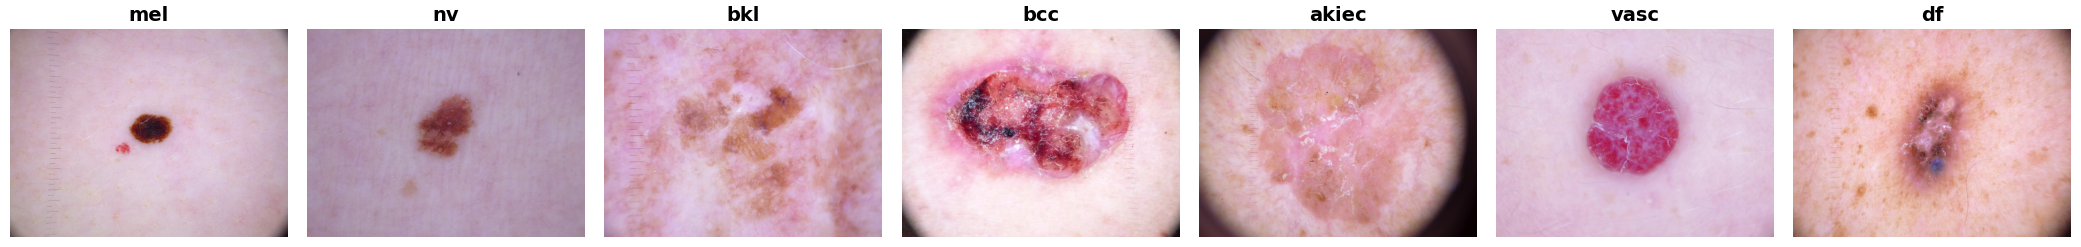
\includegraphics[width=\textwidth]{class_samples_notitle.png}
\caption{One image from each of the seven classes of HAM10000.}
\label{fig:samples}
\end{figure}

\begin{table}[!htbp]
\centering
\caption{Number of images per class in each split. The split is made over lesions.}
\label{tab:split}
\begin{tabular}{lrrr}
\toprule
Class & Train & Validation & Test \\
\midrule
mel   & 775  & 193 & 145 \\
nv    & 4728 & 958 & 1019 \\
bkl   & 734  & 180 & 185 \\
bcc   & 355  & 82  & 77 \\
akiec & 235  & 41  & 51 \\
vasc  & 85   & 41  & 16 \\
df    & 75   & 17  & 23 \\
\midrule
Total & 6987 & 1512 & 1516 \\
\bottomrule
\end{tabular}
\end{table}

\subsection{Hair Removal}

A common approach applies a black hat transform, thresholds the response and inpaints every pixel above the threshold. We call this the aggressive variant. With a $17 \times 17$ kernel and a threshold of 10, it marked a median of 12.4\% of the pixels in a sample of 300 test images, and more than 10\% of the image in 181 of them. Hair covers far less than that, so the method also repaints skin texture and lesion structure.

We therefore use a conservative variant. The grey image is smoothed lightly, a black hat transform with an $11 \times 11$ elliptical kernel is applied and the response is thresholded at 22. Connected regions are then kept only if they are shaped like a hair, meaning that their longer side is at least 35 pixels and that they are either sparse inside their bounding box (fill ratio below 0.35) or elongated (aspect ratio of at least 4). The remaining mask is dilated by one pixel and filled by the method of Telea \cite{telea2004}. Images in which no such region is found are left unchanged. On the same 300 images this variant altered a mean of 1.1\% of the pixels and left 201 images untouched. Figure~\ref{fig:hair} compares the two. Whether either variant helps accuracy is tested in the ablation.

\begin{figure}[!htbp]
\centering
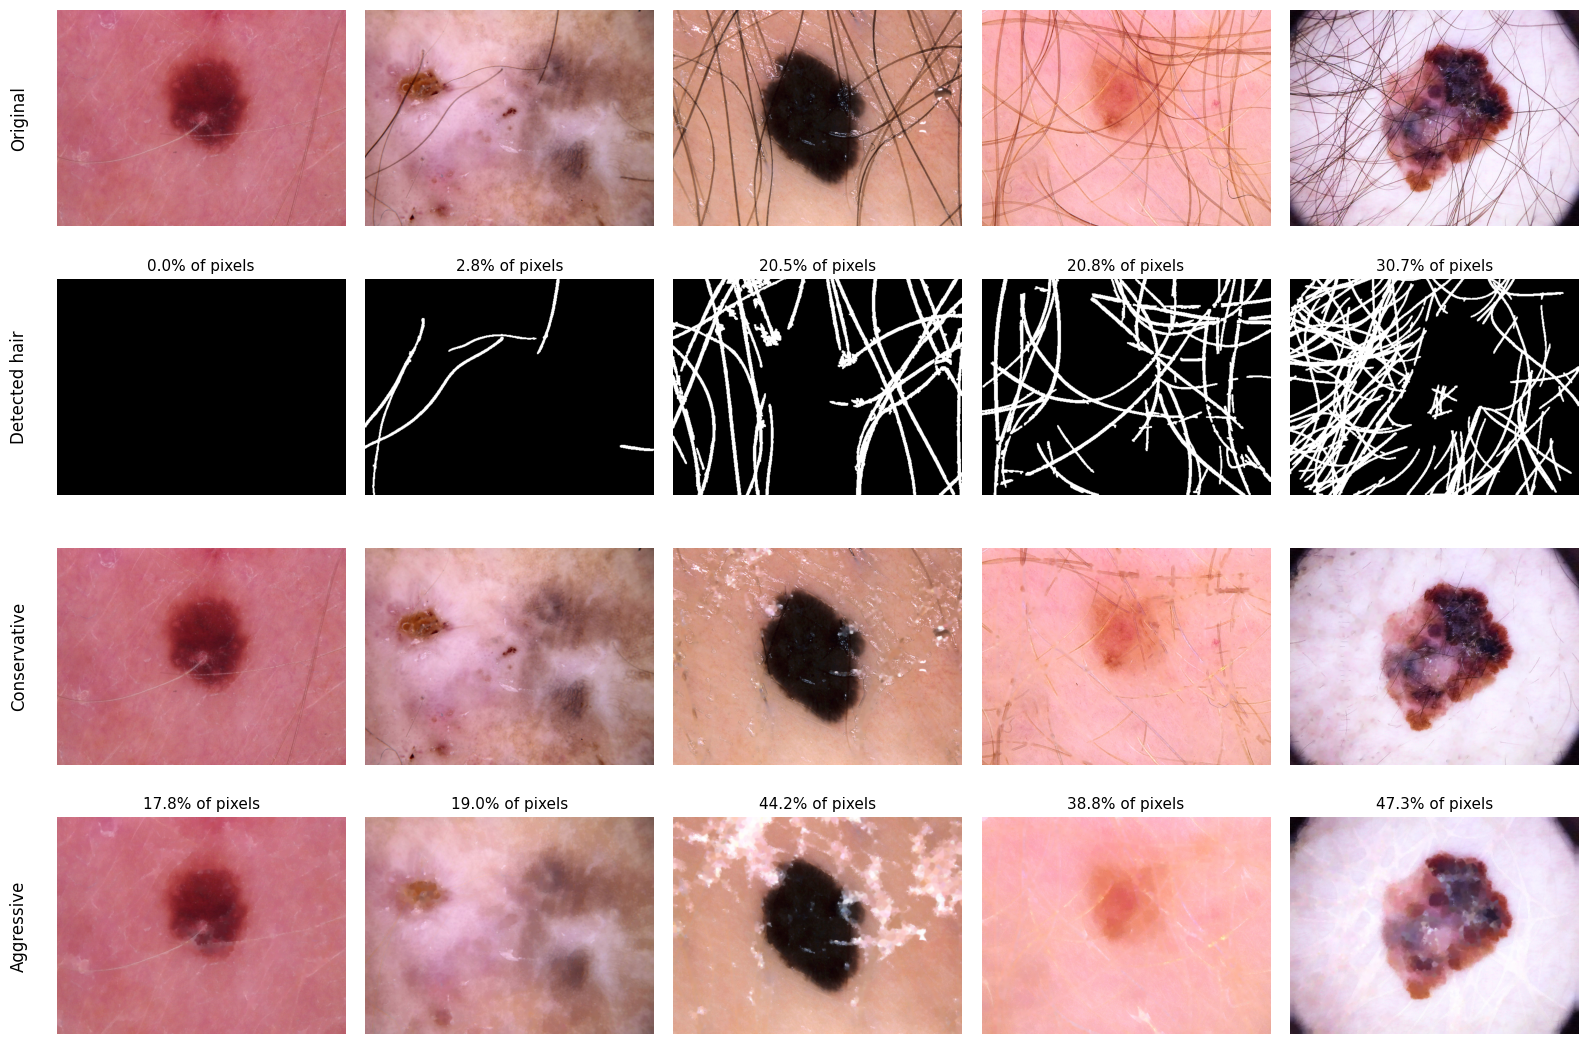
\includegraphics[width=\textwidth]{hair_comparison.png}
\caption{Hair removal on five test images. From top: original image, hair detected by the conservative variant, conservative result, aggressive result. The percentages give the share of pixels each variant repaints.}
\label{fig:hair}
\end{figure}

\subsection{Model}

Figure~\ref{fig:arch} gives an overview of the whole system, with the model in the dashed box. The backbone is the feature extractor of MobileNetV3-Small \cite{howard2019} with ImageNet weights. For a $448 \times 448$ input it produces a $14 \times 14$ map with 576 channels. Each of the 196 positions is treated as a token and projected linearly to 384 dimensions. A learnable class token is added in front and learnable position embeddings are summed with the sequence. Writing $\mathbf{f}_1, \dots, \mathbf{f}_N \in \mathbb{R}^{576}$ for the backbone features at the $N = 196$ positions, the input to the encoder is
\begin{equation}
\mathbf{Z}_0 = \left[\mathbf{c};\ \mathbf{W}\mathbf{f}_1;\ \dots;\ \mathbf{W}\mathbf{f}_N\right] + \mathbf{P},
\label{eq:tokens}
\end{equation}
where $\mathbf{W} \in \mathbb{R}^{384 \times 576}$ is the learned projection, $\mathbf{c} \in \mathbb{R}^{384}$ is the class token and $\mathbf{P} \in \mathbb{R}^{(N+1) \times 384}$ holds the position embeddings. The tokens pass through four Transformer encoder layers \cite{vaswani2017}, each with four attention heads, a feed forward width of 1536, GELU activations, layer normalisation applied before each sublayer and a dropout rate of 0.3. The final class token is normalised and mapped to seven outputs by a linear layer. The model has 8.33 million parameters, of which the Transformer accounts for about 86\%.

To measure what the Transformer contributes, we define a \emph{CNN only} variant in which the encoder is removed and the projected tokens are averaged before the same normalisation and output layer. It has 1.15 million parameters.

\begin{figure}[!htbp]
\centering
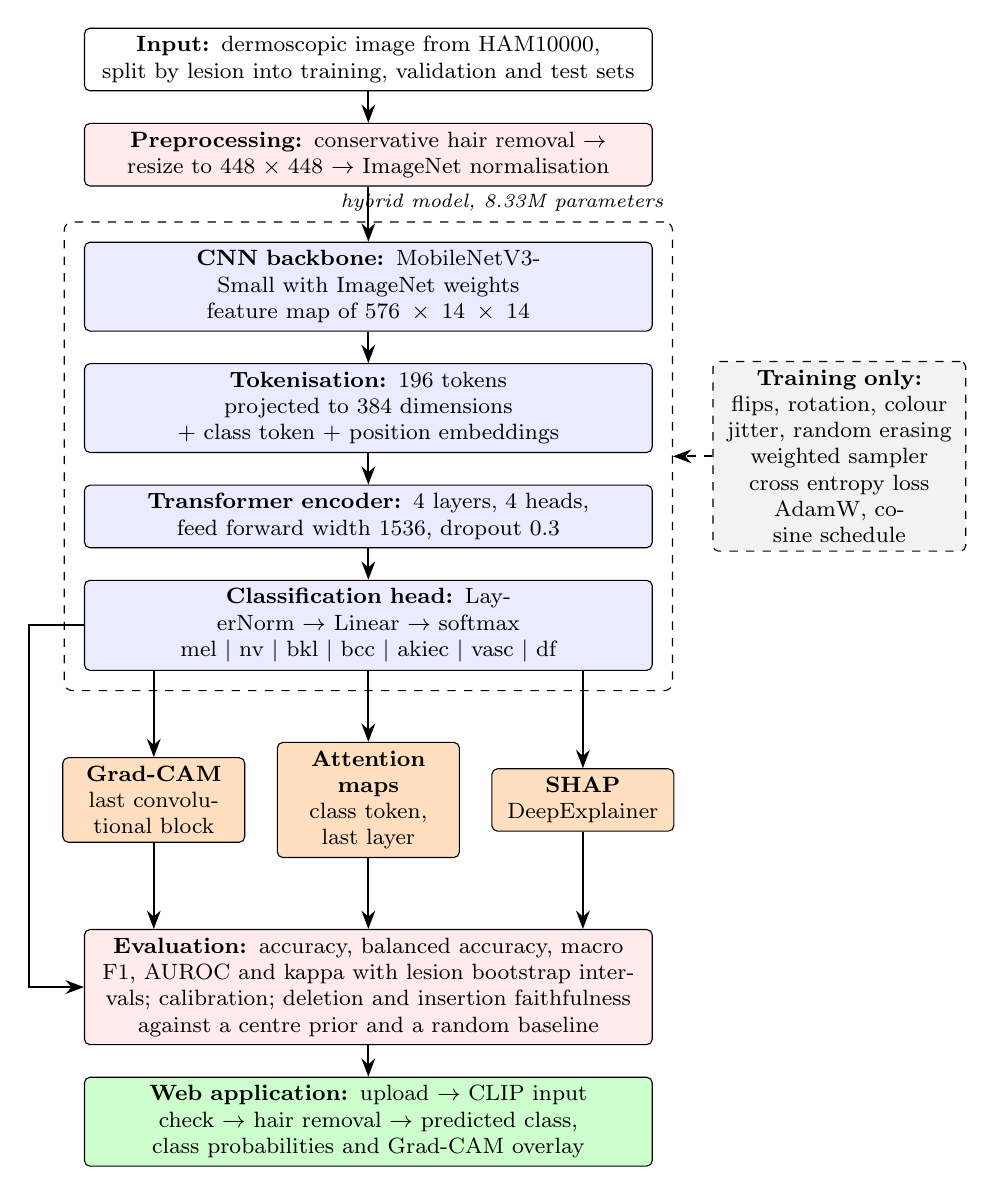
\begin{tikzpicture}[font=\footnotesize, node distance=4mm,
  box/.style={draw, rounded corners=2pt, align=center, text width=7cm, inner sep=3pt, fill=red!8},
  model/.style={box, fill=blue!8},
  xai/.style={draw, rounded corners=2pt, align=center, text width=2.1cm, inner sep=3pt, fill=orange!25},
  side/.style={draw, dashed, rounded corners=2pt, align=center, text width=3cm, inner sep=3pt, fill=gray!10},
  arr/.style={-{Stealth}, thick}]

\node[box, fill=white] (in) {\textbf{Input:} dermoscopic image from HAM10000,\\ split by lesion into training, validation and test sets};
\node[box, below=of in] (pre) {\textbf{Preprocessing:} conservative hair removal $\rightarrow$ resize to $448 \times 448$ $\rightarrow$ ImageNet normalisation};
\node[model, below=7mm of pre] (cnn) {\textbf{CNN backbone:} MobileNetV3-Small with ImageNet weights\\ feature map of $576 \times 14 \times 14$};
\node[model, below=of cnn] (tok) {\textbf{Tokenisation:} 196 tokens projected to 384 dimensions\\ + class token + position embeddings};
\node[model, below=of tok] (tr) {\textbf{Transformer encoder:} 4 layers, 4 heads,\\ feed forward width 1536, dropout 0.3};
\node[model, below=of tr] (head) {\textbf{Classification head:} LayerNorm $\rightarrow$ Linear $\rightarrow$ softmax\\ mel $|$ nv $|$ bkl $|$ bcc $|$ akiec $|$ vasc $|$ df};
\node[draw, dashed, rounded corners=3pt, inner sep=2.5mm, fit=(cnn)(tok)(tr)(head)] (grp) {};
\node[anchor=south east, font=\scriptsize\itshape] at (grp.north east) {hybrid model, 8.33M parameters};

\node[side, anchor=west] (train) at ([xshift=5mm]grp.east) {\textbf{Training only:}\\ flips, rotation, colour jitter, random erasing\\ weighted sampler\\ cross entropy loss\\ AdamW, cosine schedule};

\node[xai, below=9mm of head] (attn) {\textbf{Attention maps}\\ class token, last layer};
\node[xai, left=4mm of attn] (cam) {\textbf{Grad-CAM}\\ last convolutional block};
\node[xai, right=4mm of attn] (shap) {\textbf{SHAP}\\ DeepExplainer};

\node[box, below=9mm of attn] (eval) {\textbf{Evaluation:} accuracy, balanced accuracy, macro F1, AUROC and kappa with lesion bootstrap intervals; calibration; deletion and insertion faithfulness against a centre prior and a random baseline};
\node[box, below=of eval, fill=green!20] (app) {\textbf{Web application:} upload $\rightarrow$ CLIP input check $\rightarrow$ hair removal $\rightarrow$ predicted class, class probabilities and Grad-CAM overlay};

\draw[arr] (in) -- (pre);
\draw[arr] (pre) -- (cnn);
\draw[arr] (cnn) -- (tok);
\draw[arr] (tok) -- (tr);
\draw[arr] (tr) -- (head);
\draw[arr, dashed] (train.west) -- (grp.east);
\draw[arr] (head.south -| cam) -- (cam.north);
\draw[arr] (head.south) -- (attn.north);
\draw[arr] (head.south -| shap) -- (shap.north);
\draw[arr] (cam) -- (cam |- eval.north);
\draw[arr] (attn) -- (eval);
\draw[arr] (shap) -- (shap |- eval.north);
\draw[arr] (head.west) -- ++(-7mm,0) |- (eval.west);
\draw[arr] (eval) -- (app);
\end{tikzpicture}
\caption{Overview of the system. The dashed box is the hybrid model. The CNN only variant replaces the Transformer encoder with an average over the tokens. Augmentation and the weighted sampler are used during training only.}
\label{fig:arch}
\end{figure}

\subsection{Training}

Images are resized to the input size and augmented with random horizontal and vertical flips, rotation of up to 20 degrees, colour jitter and random erasing \cite{zhong2020}. Class imbalance is handled in one place only. Each training batch is drawn with a weighted sampler whose weights are inversely proportional to class frequency, and the loss is plain cross entropy. With $n$ training images, of which $n_k$ belong to class $k$, and $C = 7$ classes, image $i$ with label $y_i$ is drawn with probability
\begin{equation}
p_i = \frac{w_{y_i}}{\sum_{j=1}^{n} w_{y_j}}, \qquad w_k = \frac{n}{C\, n_k},
\label{eq:sampler}
\end{equation}
so that every class is seen about equally often. Combining the sampler with a class weighted loss corrects for imbalance twice, and the ablation shows that this is harmful.

All models are trained with AdamW \cite{loshchilov2019} at a learning rate of $10^{-4}$ and weight decay of $10^{-4}$, cosine annealing of the learning rate \cite{loshchilov2017} and a batch size of 16. Training stops when the validation loss has not improved for a set number of epochs, and the weights with the lowest validation loss are kept. The main model is trained at 448 pixels for up to 50 epochs with a patience of 10. Experiments were run in PyTorch \cite{paszke2019} on a single Tesla T4 GPU.

\subsection{Comparison Models and Protocol}

EfficientNet-B3 \cite{tan2019} and ViT-B/16 \cite{dosovitskiy2021} represent a strong compact CNN and a standard Transformer. Both are taken from torchvision with ImageNet weights and a new seven class output layer. ViT-B/16 requires a $224 \times 224$ input, so 224 pixels is the one size that all models share. The hybrid, the CNN only variant, EfficientNet-B3 and ViT-B/16 are each trained at that size with the same preprocessing, augmentation, sampler, loss, optimiser, limit of 20 epochs and patience of 5, and each is trained three times with different seeds. We did not train the comparison models at 448 pixels for reasons of compute, so the main model is never set against them directly.

\subsection{Evaluation}

We report accuracy, balanced accuracy \cite{brodersen2010}, which was also the ranking metric of the ISIC 2018 challenge \cite{codella2019}, macro averaged F1, macro averaged one versus rest AUROC and Cohen's kappa \cite{cohen1960}. With $m$ test images, $m_k$ of class $k$ and $t_k$ of those classified correctly, balanced accuracy is the mean recall over classes and kappa corrects accuracy for chance agreement:
\begin{equation}
\mathrm{BA} = \frac{1}{C} \sum_{k=1}^{C} \frac{t_k}{m_k}, \qquad \kappa = \frac{p_o - p_e}{1 - p_e},
\label{eq:metrics}
\end{equation}
where $p_o$ is the accuracy and $p_e$ is the agreement expected by chance from the frequencies of the true and predicted labels. The unweighted form of kappa is used because the classes have no natural order. Confidence intervals at the 95\% level come from 2,000 bootstrap resamples \cite{efron1993} in which whole lesions are drawn, since images of one lesion are not independent. Differences between two models are evaluated on the same resamples. These intervals describe uncertainty from the test sample. Variation between training runs is shown separately by the spread over seeds. Calibration is summarised by the expected calibration error \cite{guo2017}. The test images are grouped into $B = 15$ bins by the probability of their predicted class, and
\begin{equation}
\mathrm{ECE} = \sum_{b=1}^{B} \frac{|S_b|}{m} \left| \mathrm{acc}(S_b) - \mathrm{conf}(S_b) \right|,
\label{eq:ece}
\end{equation}
where $S_b$ is the set of images in bin $b$, $\mathrm{acc}(S_b)$ is the fraction of them classified correctly and $\mathrm{conf}(S_b)$ is their mean predicted probability.

Because the sampler presents the classes in equal proportion, the model may predict rare classes more often than their true frequency warrants. We therefore also test a correction in the manner of logit adjustment \cite{menon2021}. With $q_k(x)$ the predicted probability of class $k$ for image $x$ and $\pi_k$ the frequency of class $k$ in the training set, the adjusted prediction is
\begin{equation}
\hat{y}(x) = \arg\max_{k} \left[ \log q_k(x) + \tau \log \pi_k \right],
\label{eq:prior}
\end{equation}
where $\tau \ge 0$ sets the strength and $\tau = 0$ leaves the model unchanged. The value of $\tau$ is chosen on the validation set.

\subsection{Explainability}

Three kinds of explanation are produced for the main model. Grad-CAM \cite{selvaraju2017} is computed on the last convolutional block. SHAP values are estimated with DeepExplainer \cite{lundberg2017} using 30 background images. Attention maps are taken from the class token of the last Transformer layer, averaged over heads.

To test faithfulness we follow Petsiuk et al.\ \cite{petsiuk2018}. In the deletion test the pixels ranked most important are replaced by the dataset mean in 20 steps and the probability of the predicted class is recorded, so a faithful map makes it fall quickly and gives a small area under the curve. In the insertion test the pixels are added in the same order to a blurred copy of the image, so a faithful map gives a large area. Because lesions are centred, we compare each method with a fixed Gaussian centred on the image, which we call the centre prior, and with random noise. The test uses up to 25 test images per class, 164 in total, and paired Wilcoxon signed rank tests \cite{wilcoxon1945}. SHAP is shown qualitatively only.

\subsection{Few Shot and Zero Shot Experiments}

For few shot classification of the three rarest classes (df, vasc and akiec), a class prototype is the mean embedding of a few training images and a test image is assigned to the nearest prototype \cite{snell2017}. If $g(x)$ denotes the embedding of image $x$ and $S_k$ the set of $s$ support images of class $k$, then
\begin{equation}
\boldsymbol{\mu}_k = \frac{1}{s} \sum_{x_i \in S_k} g(x_i), \qquad \hat{y}(x) = \arg\min_{k} \left\lVert g(x) - \boldsymbol{\mu}_k \right\rVert_2 .
\label{eq:proto}
\end{equation}
We use $s = 1$, 5 and 10 and average over 200 random episodes with 15 test queries per class. Three embeddings are compared: the main model, which has seen these classes, MobileNetV3-Small with ImageNet weights only, and a hybrid trained on the other four classes, for which the three rare classes are unseen. Zero shot classification uses CLIP ViT-B/32 \cite{radford2021} with one text description per class. The same CLIP model is also used in our demonstration application as a check that an uploaded image is a skin lesion at all, by comparing a lesion prompt with a prompt describing ordinary photographs. We evaluate that check on the test set and on 300 images from CIFAR-10 \cite{krizhevsky2009}.

\subsection{Demonstration Application}

The trained model is wrapped in a small web application built with Streamlit. A user uploads an image, and the application first applies the CLIP input check described above \cite{radford2021}. If the image does not appear to be a dermoscopic lesion, the user is warned and may choose to continue anyway. The application then applies the same conservative hair removal used in training and shows the predicted class, the probability of every class and a Grad-CAM overlay. It is intended to demonstrate the pipeline and carries a notice that it is not validated for clinical use.

\section{Results}

\subsection{Main Model}

The main model stopped after 18 epochs, with the best validation loss at epoch 8 (Fig.~\ref{fig:curves}). Table~\ref{tab:main} gives its test results beside those of the CNN only variant trained in the same way. The hybrid is well above the majority baseline of 0.672 in accuracy. Against the CNN only variant it is higher in accuracy by 0.036, and the interval for that difference, 0.014 to 0.058, excludes zero (Table~\ref{tab:paired}). On balanced accuracy, macro F1 and AUROC the CNN only variant is slightly higher and the intervals for the differences include zero. The two models make different trade offs more than they differ in quality. The hybrid assigns more images to nevus, which raises accuracy on a test set dominated by that class, while the CNN only variant recovers more of the melanomas, benign keratoses and basal cell carcinomas. Each model was trained once at this size, so these differences should be read with care.

\begin{table}[!htbp]
\centering
\caption{Test results at 448 pixels with 95\% lesion bootstrap intervals. Always predicting nevus gives an accuracy of 0.672.}
\label{tab:main}
\small
\begin{tabular}{lcc}
\toprule
 & Hybrid & CNN only \\
\midrule
Parameters (millions) & 8.33 & 1.15 \\
Accuracy & 0.821 (0.796 to 0.844) & 0.784 (0.760 to 0.808) \\
Balanced accuracy & 0.729 (0.677 to 0.779) & 0.743 (0.692 to 0.790) \\
Macro F1 & 0.699 (0.644 to 0.740) & 0.711 (0.658 to 0.751) \\
Macro AUROC & 0.946 (0.918 to 0.964) & 0.952 (0.935 to 0.966) \\
Cohen's kappa & 0.657 (0.612 to 0.697) & 0.621 (0.580 to 0.660) \\
\bottomrule
\end{tabular}
\end{table}

\begin{figure}[!htbp]
\centering
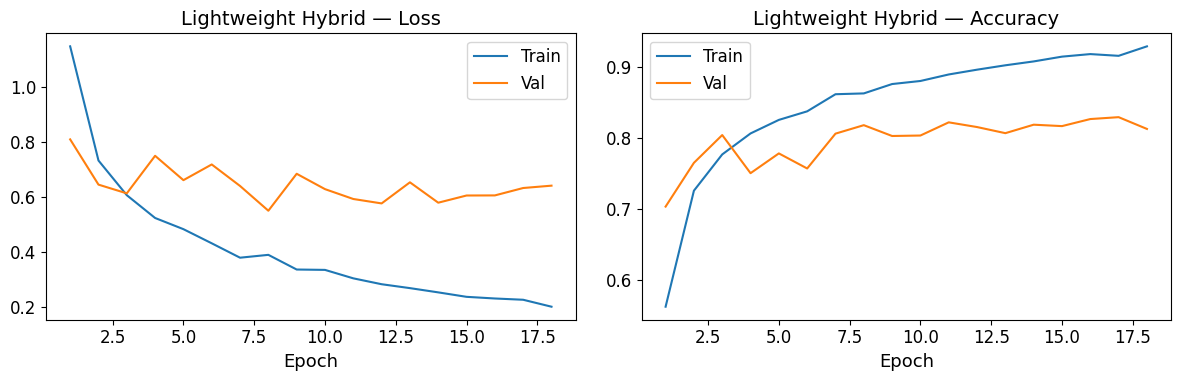
\includegraphics[width=\textwidth]{training_curves.png}
\caption{Training and validation loss and accuracy of the main model. The saved weights are those of epoch 8.}
\label{fig:curves}
\end{figure}

\subsection{Comparison under an Equal Budget}

Table~\ref{tab:seeds} reports the mean and standard deviation over three seeds at 224 pixels, and Fig.~\ref{fig:allcurves} shows the training curves of all four models for the first seed. In every model the training loss keeps falling while the validation loss flattens, the usual sign of overfitting, and the weights that are kept are those with the lowest validation loss.

EfficientNet-B3 is the best model on every metric. It scores above the hybrid on all five metrics in each of the three seeds, and the two sets of runs do not overlap on any metric. For the first seed (Table~\ref{tab:paired}), its advantage over the hybrid is 0.059 in accuracy, 0.102 in macro F1 and 0.024 in AUROC, and the bootstrap intervals for those metrics and for kappa exclude zero. The interval for balanced accuracy, a difference of 0.047, only just reaches zero.

The hybrid and ViT-B/16 are close, with a consistent pattern. ViT-B/16 is higher on accuracy, macro F1 and kappa in all three seeds, and the hybrid is higher on balanced accuracy in all three. The hybrid therefore does better on the rare classes and worse on the frequent one. For the first seed every interval for their difference includes zero. The hybrid reaches this level with 8.3 million parameters against 85.8 million.

The CNN only variant is slightly ahead of the hybrid on every mean, and it is higher on accuracy, macro F1 and kappa in all three seeds, although the two sets of runs overlap on every metric. For the first seed its advantage in accuracy (0.023) and kappa (0.046) is supported by intervals that exclude zero. There is therefore no evidence that the Transformer helps at this resolution, and some evidence that it costs a little. Comparing Tables~\ref{tab:main} and~\ref{tab:seeds}, doubling the input size raises the hybrid's accuracy from about 0.75 to 0.82 and its macro F1 from about 0.63 to 0.70, although the two settings also differ in their epoch limits.

\begin{table}[!htbp]
\centering
\caption{Paired differences on the test set, hybrid minus the named model, with 95\% lesion bootstrap intervals in brackets. Negative values favour the named model. The 224 pixel columns use the first seed.}
\label{tab:paired}
\footnotesize\setlength{\tabcolsep}{4pt}
\begin{tabular}{lcccc}
\toprule
 & 448 px & \multicolumn{3}{c}{224 px} \\
\cmidrule(lr){2-2}\cmidrule(lr){3-5}
Metric & CNN only & CNN only & EfficientNet-B3 & ViT-B/16 \\
\midrule
Accuracy  & $+0.036$ & $-0.023$ & $-0.059$ & $-0.005$ \\
          & $[+0.014, +0.058]$ & $[-0.041, -0.005]$ & $[-0.084, -0.035]$ & $[-0.028, +0.020]$ \\
Bal.\ acc. & $-0.014$ & $-0.025$ & $-0.047$ & $+0.027$ \\
          & $[-0.047, +0.021]$ & $[-0.059, +0.011]$ & $[-0.095, -0.000]$ & $[-0.036, +0.082]$ \\
Macro F1  & $-0.012$ & $-0.035$ & $-0.102$ & $-0.022$ \\
          & $[-0.051, +0.025]$ & $[-0.069, -0.000]$ & $[-0.149, -0.053]$ & $[-0.079, +0.035]$ \\
AUROC     & $-0.006$ & $-0.003$ & $-0.024$ & $-0.006$ \\
          & $[-0.024, +0.006]$ & $[-0.010, +0.004]$ & $[-0.041, -0.009]$ & $[-0.023, +0.007]$ \\
Kappa     & $+0.036$ & $-0.046$ & $-0.098$ & $-0.018$ \\
          & $[-0.002, +0.072]$ & $[-0.076, -0.015]$ & $[-0.138, -0.056]$ & $[-0.056, +0.024]$ \\
\bottomrule
\end{tabular}
\end{table}

\begin{figure}[!htbp]
\centering
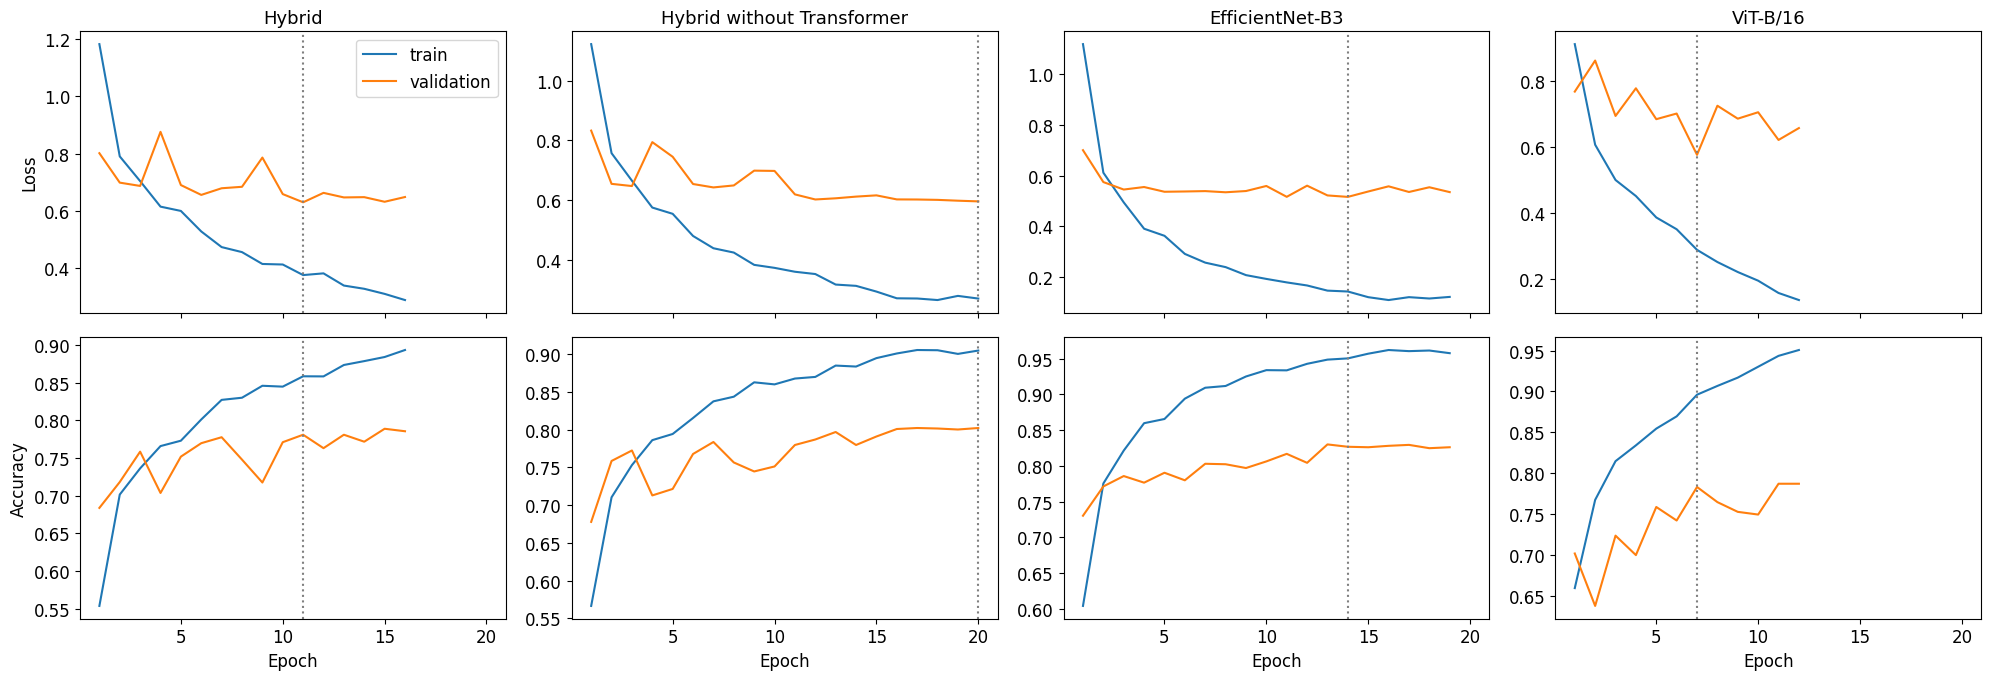
\includegraphics[width=\textwidth]{curves_all_models.png}
\caption{Training and validation curves at 224 pixels for the first seed (top: loss, bottom: accuracy). The dotted line marks the epoch whose weights were kept. The second panel is the CNN only variant.}
\label{fig:allcurves}
\end{figure}

\begin{table}[!htbp]
\centering
\caption{Test results at 224 pixels under an identical pipeline, mean $\pm$ standard deviation over three seeds.}
\label{tab:seeds}
\small\setlength{\tabcolsep}{4pt}
\begin{tabular}{lcccc}
\toprule
Metric & EfficientNet-B3 & ViT-B/16 & CNN only & Hybrid \\
\midrule
Accuracy    & $0.814 \pm 0.014$ & $0.782 \pm 0.015$ & $0.773 \pm 0.017$ & $0.751 \pm 0.030$ \\
Bal.\ acc.  & $0.718 \pm 0.014$ & $0.649 \pm 0.004$ & $0.693 \pm 0.016$ & $0.682 \pm 0.007$ \\
Macro F1    & $0.714 \pm 0.026$ & $0.661 \pm 0.022$ & $0.662 \pm 0.018$ & $0.630 \pm 0.019$ \\
AUROC       & $0.957 \pm 0.005$ & $0.942 \pm 0.007$ & $0.941 \pm 0.002$ & $0.935 \pm 0.008$ \\
Kappa       & $0.651 \pm 0.025$ & $0.598 \pm 0.013$ & $0.592 \pm 0.024$ & $0.555 \pm 0.040$ \\
Parameters (millions) & 10.71 & 85.80 & 1.15 & 8.27 \\
\bottomrule
\end{tabular}
\end{table}

\subsection{Ablation}

Table~\ref{tab:ablation} changes one element of the pipeline at a time, at 224 pixels with a single seed. With one seed, differences of about 0.02 in balanced accuracy are within the variation seen between seeds in Table~\ref{tab:seeds}, and we do not interpret them.

Pretraining has the largest effect. Without ImageNet weights, balanced accuracy falls from 0.679 to 0.535 and macro F1 from 0.638 to 0.420. The aggressive hair removal is also clearly harmful, lowering balanced accuracy to 0.605 and macro F1 to 0.510. Training on the original images gives results within noise of the conservative variant, so careful hair removal does no harm but is not shown to help.

The imbalance rows explain a failure that is easy to miss. Adding a class weighted loss on top of the sampler lifts balanced accuracy slightly to 0.695 but drops accuracy to 0.575, which is below the majority baseline, because the model then over predicts the rare classes. Using the weighted loss alone performs about as well as the sampler alone. Using neither gives the highest accuracy, 0.808, but a balanced accuracy of only 0.611, because the rare classes are then neglected. Halving the resolution to 112 pixels costs only a little here, and removing the Transformer does not reduce any metric.

\begin{table}[!htbp]
\centering
\caption{Ablation at 224 pixels, one seed. Each row changes one element of the reference pipeline.}
\label{tab:ablation}
\small\setlength{\tabcolsep}{4pt}
\begin{tabular}{lccccc}
\toprule
Configuration & Accuracy & Bal.\ acc. & Macro F1 & AUROC & Kappa \\
\midrule
Reference                    & 0.763 & 0.679 & 0.638 & 0.939 & 0.568 \\
No pretraining               & 0.631 & 0.535 & 0.420 & 0.892 & 0.405 \\
Sampler and weighted loss    & 0.575 & 0.695 & 0.521 & 0.902 & 0.390 \\
Weighted loss only           & 0.776 & 0.702 & 0.653 & 0.943 & 0.602 \\
No imbalance handling        & 0.808 & 0.611 & 0.636 & 0.948 & 0.619 \\
CNN only (no Transformer)    & 0.786 & 0.704 & 0.673 & 0.942 & 0.614 \\
No hair removal              & 0.749 & 0.690 & 0.645 & 0.932 & 0.562 \\
Aggressive hair removal      & 0.685 & 0.605 & 0.510 & 0.922 & 0.464 \\
Input size 112               & 0.739 & 0.666 & 0.610 & 0.930 & 0.542 \\
\bottomrule
\end{tabular}
\end{table}

\subsection{Efficiency}

Table~\ref{tab:eff} lists size, computation and latency for one image. The hybrid at 448 pixels needs more floating point operations than EfficientNet-B3 at 224 pixels but is faster on both devices, and it is smaller in parameters. It is far lighter than ViT-B/16 on every measure. The CNN only variant is the cheapest by a wide margin. The word lightweight is therefore justified for the hybrid in size and latency relative to the comparison models, but the Transformer is responsible for most of its cost.

\begin{table}[!htbp]
\centering
\caption{Efficiency for a single image. FLOPs count multiplications and additions separately. Latency is the median on a Tesla T4 GPU and on the host CPU.}
\label{tab:eff}
\small
\begin{tabular}{lcrrrr}
\toprule
Model & Input & Params (M) & GFLOPs & GPU (ms) & CPU (ms) \\
\midrule
Hybrid          & 448 & 8.33  & 3.31  & 8.1  & 51 \\
CNN only        & 448 & 1.15  & 0.52  & 5.2  & 19 \\
Hybrid          & 224 & 8.27  & 0.84  & 6.6  & 20 \\
CNN only        & 224 & 1.15  & 0.13  & 5.4  & 9 \\
EfficientNet-B3 & 224 & 10.71 & 1.92  & 12.8 & 65 \\
ViT-B/16        & 224 & 85.80 & 33.70 & 19.1 & 482 \\
\bottomrule
\end{tabular}
\end{table}

\subsection{Explanations}

Figures~\ref{fig:gradcam}, \ref{fig:attn} and~\ref{fig:shap} show Grad-CAM, attention and SHAP maps for one test image per class. For most classes the Grad-CAM map falls on part of the lesion. For the nevus example it is weak over the lesion, and in several images it also responds to the corners of the frame, including the dark border left by the dermoscope, which are not part of the lesion at all. The attention maps concentrate on a few tokens near the middle of the lesion, except for the nevus example where attention is spread widely. The SHAP maps are diffuse and centred. Such pictures cannot settle whether the model relies on the lesion, since a map on the centre is expected for centred images in any case. Table~\ref{tab:xai} gives the faithfulness test. On insertion, Grad-CAM (0.694) and attention (0.641) are both significantly better than the centre prior (0.594), with $p < 0.0001$ in each case. On deletion, neither differs from the centre prior ($p = 0.99$ and $p = 0.61$), Grad-CAM gives a lower area than the centre prior in only 46\% of images, and random noise has the lowest area of all. A likely reason is that scattered random deletion disturbs the image everywhere at once, which can lower confidence faster than removing a compact region, so the deletion test is less informative for this model. The fair conclusion is that the maps identify regions that are sufficient to restore the prediction more efficiently than a centre blob does, but the evidence that those regions are necessary is absent.

\begin{figure}[!htbp]
\centering
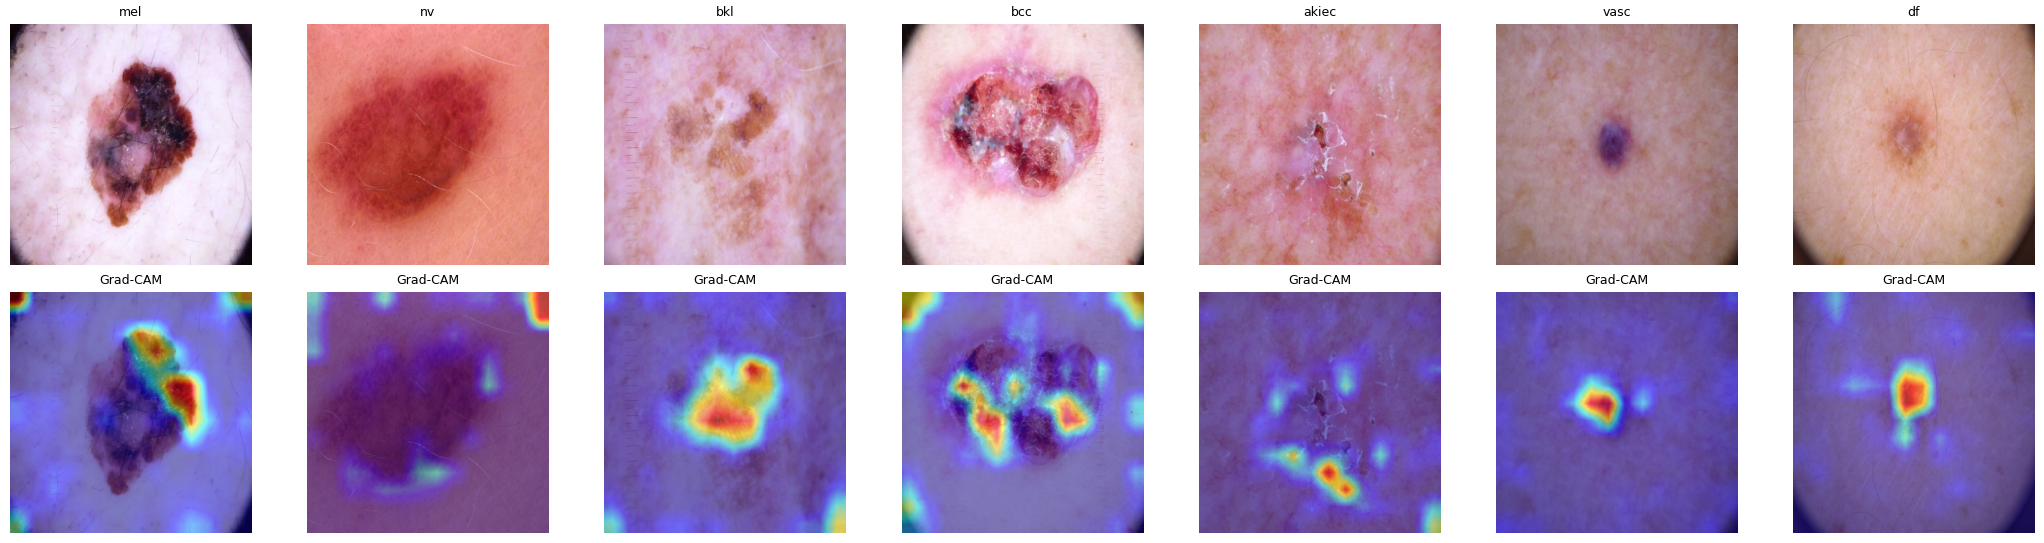
\includegraphics[width=\textwidth]{gradcam_notitle.png}
\caption{Grad-CAM for one test image per class (top: image, bottom: overlay).}
\label{fig:gradcam}
\end{figure}

\begin{figure}[!htbp]
\centering
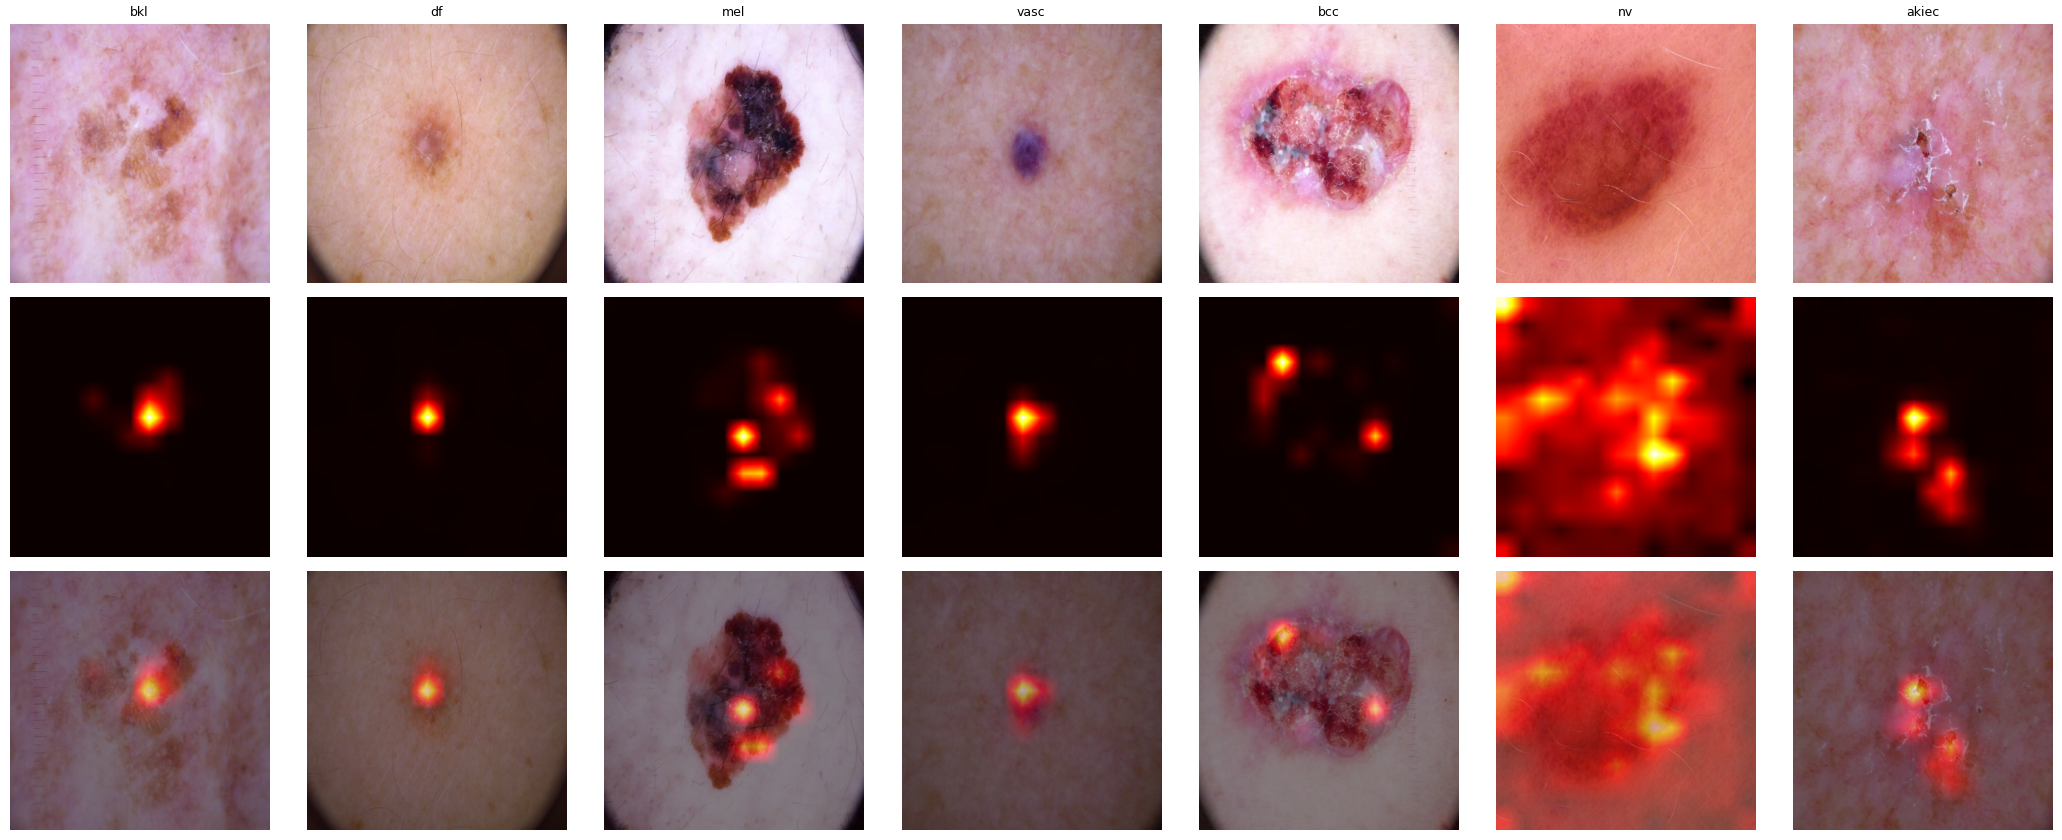
\includegraphics[width=\textwidth]{attention_maps_notitle.png}
\caption{Attention of the class token in the last Transformer layer, averaged over heads (top: image, middle: attention, bottom: overlay).}
\label{fig:attn}
\end{figure}

\begin{figure}[!htbp]
\centering
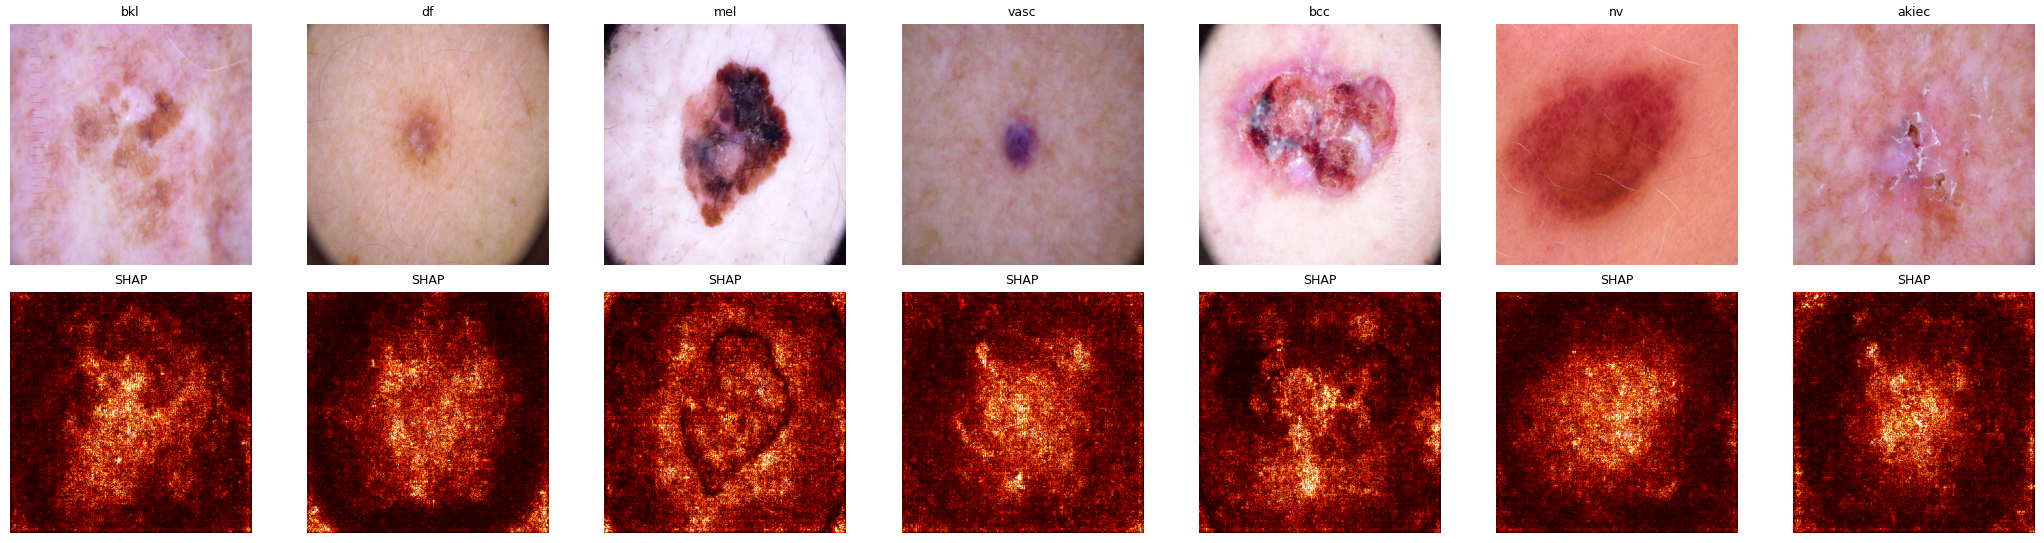
\includegraphics[width=\textwidth]{shap_notitle.png}
\caption{SHAP attributions for the same images as Fig.~\ref{fig:attn} (top: image, bottom: mean absolute attribution).}
\label{fig:shap}
\end{figure}

\begin{table}[!htbp]
\centering
\caption{Faithfulness of explanations on 164 test images, mean area under the curve. Lower is better for deletion and higher is better for insertion.}
\label{tab:xai}
\begin{tabular}{lcc}
\toprule
Method & Deletion & Insertion \\
\midrule
Grad-CAM     & 0.302 & 0.694 \\
Attention    & 0.296 & 0.641 \\
Centre prior & 0.311 & 0.594 \\
Random       & 0.245 & 0.381 \\
\bottomrule
\end{tabular}
\end{table}

\subsection{Clinical Reading and Calibration}

Table~\ref{tab:clin} breaks the main model's results down by class, and Fig.~\ref{fig:cm} gives the confusion matrix. Nevus is recognised reliably. Melanoma has a sensitivity of 0.566 and a positive predictive value of 0.550. Of 145 melanomas, 43 were classified as nevus, while 48 of 1,019 nevi were classified as melanoma. Grouping melanoma and basal cell carcinoma as cancer gives a sensitivity of 0.631 and a specificity of 0.931, and the AUROC for melanoma against all other classes is 0.899. A kappa of 0.657 falls in the range conventionally described as substantial agreement \cite{landis1977}, but the melanoma sensitivity is too low for the model to be used for screening as it stands.

\begin{figure}[!htbp]
\centering
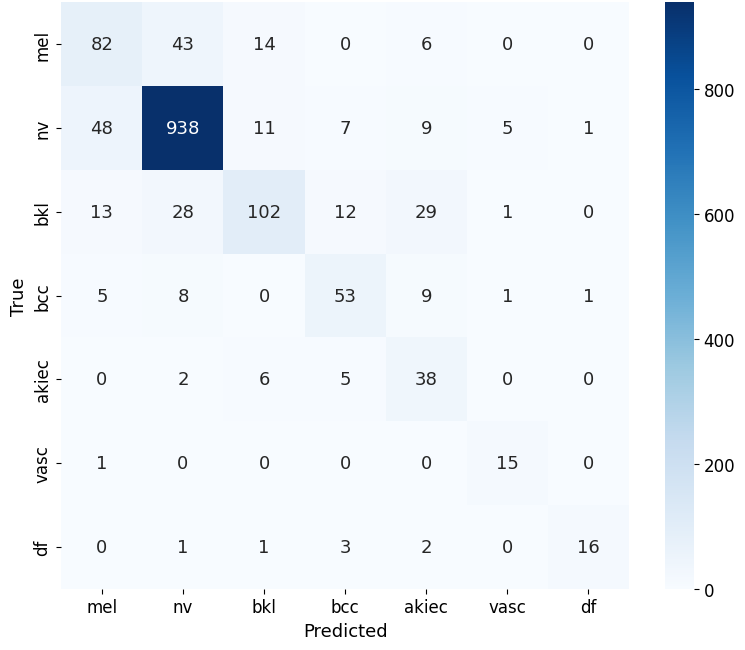
\includegraphics[width=0.62\textwidth]{confusion_matrix_notitle.png}
\caption{Confusion matrix of the main model on the test set (rows: reference diagnosis, columns: prediction).}
\label{fig:cm}
\end{figure}

The expected calibration error is 0.053, so the predicted probabilities are close to the observed frequencies. The reliability diagram in Fig.~\ref{fig:rel} shows where the remaining error lies: predictions made with a probability between about 0.6 and 0.9 are correct somewhat less often than the probability suggests.

\begin{figure}[!htbp]
\centering
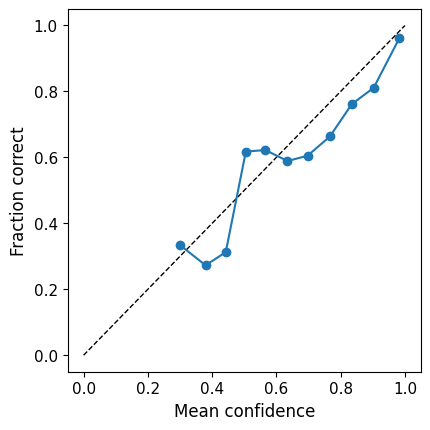
\includegraphics[width=0.42\textwidth]{reliability.png}
\caption{Reliability diagram of the main model on the test set. The dashed line is perfect calibration.}
\label{fig:rel}
\end{figure}

The prior adjustment of Eq.~\eqref{eq:prior}, with $\tau = 0.4$ chosen on the validation set, raised test accuracy slightly, from 0.821 to 0.828, but reduced melanoma sensitivity from 0.566 to 0.448, so we do not adopt it.

\begin{table}[!htbp]
\centering
\caption{Per class results of the main model on the test set.}
\label{tab:clin}
\begin{tabular}{lrcccc}
\toprule
Class & $n$ & Sensitivity & Specificity & PPV & NPV \\
\midrule
mel   & 145  & 0.57 & 0.95 & 0.55 & 0.95 \\
nv    & 1019 & 0.92 & 0.84 & 0.92 & 0.84 \\
bkl   & 185  & 0.55 & 0.98 & 0.76 & 0.94 \\
bcc   & 77   & 0.69 & 0.98 & 0.66 & 0.98 \\
akiec & 51   & 0.75 & 0.96 & 0.41 & 0.99 \\
vasc  & 16   & 0.94 & 1.00 & 0.68 & 1.00 \\
df    & 23   & 0.70 & 1.00 & 0.89 & 1.00 \\
\bottomrule
\end{tabular}
\end{table}

\subsection{Few Shot, Zero Shot and the Input Check}

Table~\ref{tab:fewshot} gives the few shot results. With the main model as the embedding, three way accuracy on the rare classes is about 90\% whatever the number of examples, but this model was trained on those classes and the figure does not measure generalisation. When the three classes are withheld from training, accuracy rises from 47.4\% with one example to 65.6\% with ten, against 44.8\% and 62.0\% for ImageNet features alone and a chance level of 33.3\%. Training on the other skin lesion classes therefore adds only a few points over generic features.

\begin{table}[!htbp]
\centering
\caption{Three way few shot accuracy (\%) on df, vasc and akiec: mean over 200 episodes, with the range that contains 95\% of episodes in brackets. The unseen row is a hybrid trained without these three classes. Chance is 33.3\%.}
\label{tab:fewshot}
\small\setlength{\tabcolsep}{4pt}
\begin{tabular}{lccc}
\toprule
Embedding & 1 example & 5 examples & 10 examples \\
\midrule
Main model (classes seen) & 89.6 [82.2, 93.3] & 90.3 [86.6, 95.6] & 90.5 [86.7, 95.6] \\
Hybrid (classes unseen)   & 47.4 [26.7, 68.9] & 60.7 [42.2, 75.6] & 65.6 [51.1, 77.8] \\
ImageNet features only    & 44.8 [31.1, 60.0] & 55.8 [40.0, 71.1] & 62.0 [46.7, 75.6] \\
\bottomrule
\end{tabular}
\end{table}

CLIP without any training reaches a balanced accuracy of 0.278 and an accuracy of 0.501 on the full test set. On the 90 test images of the three rare classes its balanced accuracy is 0.361, against 0.793 for the main model on the same images. As an input check, CLIP accepted 98.2\% of the test images as lesions (interval 0.974 to 0.988) but rejected only 52.0\% of the CIFAR-10 photographs (interval 0.464 to 0.576). The check rarely blocks genuine lesions, but it cannot be relied on to stop unrelated images.

\section{Discussion}

The clearest lessons concern the training pipeline, not the architecture. Pretraining was worth about 0.14 in balanced accuracy. Correcting for imbalance twice produced a model that looked reasonable on balanced accuracy and AUROC while performing worse than always predicting the majority class, which shows why plain accuracy and the majority baseline should be reported beside balanced metrics. A standard hair removal recipe, applied without checking how much it changes, lowered macro F1 by 0.13. None of these effects depends on the choice of backbone, and each is comparable to or larger than the differences between the architectures we compared.

On architecture, the evidence does not favour the Transformer. At 224 pixels the CNN only variant matched or exceeded the hybrid on every mean, and was ahead on accuracy, macro F1 and kappa in each of the three seeds. At 448 pixels the hybrid was more accurate, and that one difference is supported by its interval, but it was behind on balanced accuracy, macro F1 and AUROC, and each model was trained once. A plausible reading is that a pretrained CNN already captures what is needed from a centred lesion, and that with about 7,000 training images the encoder has too little data to add useful global reasoning. The practical consequence is that a model of 1.15 million parameters is a credible alternative to the hybrid, and that EfficientNet-B3 remains the better choice when accuracy matters most and its cost is acceptable.

Our numbers are lower than the best reported on HAM10000 \cite{codella2019,haque2026}. Part of the gap is to be expected, since those figures come from the leading entries of an international challenge and from a far larger network. Part reflects evaluation: we split by lesion, train one compact model and report balanced metrics. We consider the lower figures a more realistic estimate of what a compact model achieves on unseen lesions.

For explanations, the insertion result shows that Grad-CAM and attention carry information beyond the position of the lesion, which a set of example heatmaps could not establish. The deletion result shows the limits of that claim. Neither test says whether the highlighted regions correspond to features a dermatologist would use, such as those of the ABCD rule \cite{nachbar1994}, and we make no such claim.

\subsection{Limitations}

All experiments use one dataset, collected mainly from patients with lighter skin, and performance on other populations is likely to be lower \cite{daneshjou2022}. The choice of sampler and hair removal was informed by earlier experiments evaluated on the same test split, so the reported figures may be mildly optimistic. The two models at 448 pixels were each trained with one seed, and the comparison models were not trained at that size. The ablation uses one seed per row. The explanations were not reviewed by clinicians. Finally, the melanoma sensitivity of 0.566 and the weak rejection rate of the input check mean that the accompanying application is a research demonstration only.

\section{Conclusion}

We evaluated a lightweight hybrid of MobileNetV3-Small and a Transformer encoder for seven class dermoscopic classification under a protocol designed to make its claims checkable. With a lesion level split, a single correction for class imbalance and conservative hair removal, the hybrid reaches an accuracy of 0.821 and a macro AUROC of 0.946 at 448 pixels with 8.3 million parameters and good calibration. Under an equal budget it is close to ViT-B/16 at a tenth of the size, with higher balanced accuracy and lower accuracy, and it is behind EfficientNet-B3 on every metric. Its Transformer makes up most of its parameters but is not shown to improve it, and a CNN only variant with 1.15 million parameters performs similarly. Explanations from Grad-CAM and attention pass an insertion test against a centre prior and fail to separate from it on deletion. Future work should repeat the high resolution comparison with several seeds, evaluate on external data with a wider range of skin tones, improve melanoma sensitivity, and involve dermatologists in judging the explanations.

\begin{credits}
\subsubsection{Declaration of the use of AI.}
The authors used Claude (Anthropic), an AI assistant, during this project. It was used to review and correct the experiment code, to help assemble the final notebook and the demonstration application, to check the reference list against bibliographic databases, and to produce a first draft of the text of this paper from the results of the experiments. All experiments were run by the first author, and all reported numbers come from those runs. The authors reviewed and edited the text and take full responsibility for the content of the paper.

\subsubsection{\discintname}
The authors have no competing interests to declare that are relevant to the content of this article.
\end{credits}

\begin{thebibliography}{99}

\bibitem{adebayo2018}
Adebayo, J., Gilmer, J., Muelly, M., Goodfellow, I., Hardt, M., Kim, B.: Sanity checks for saliency maps. In: Advances in Neural Information Processing Systems, vol. 31 (2018)

\bibitem{brodersen2010}
Brodersen, K.H., Ong, C.S., Stephan, K.E., Buhmann, J.M.: The balanced accuracy and its posterior distribution. In: 20th International Conference on Pattern Recognition, pp. 3121--3124. IEEE (2010)

\bibitem{chen2021}
Chen, J., Lu, Y., Yu, Q., Luo, X., Adeli, E., Wang, Y., Lu, L., Yuille, A.L., Zhou, Y.: TransUNet: Transformers make strong encoders for medical image segmentation. arXiv preprint arXiv:2102.04306 (2021)

\bibitem{codella2019}
Codella, N., Rotemberg, V., Tschandl, P., Celebi, M.E., Dusza, S., Gutman, D., Helba, B., Kalloo, A., Liopyris, K., Marchetti, M., Kittler, H., Halpern, A.: Skin lesion analysis toward melanoma detection 2018: A challenge hosted by the International Skin Imaging Collaboration (ISIC). arXiv preprint arXiv:1902.03368 (2019)

\bibitem{cohen1960}
Cohen, J.: A coefficient of agreement for nominal scales. Educational and Psychological Measurement \textbf{20}(1), 37--46 (1960)

\bibitem{daneshjou2022}
Daneshjou, R., Vodrahalli, K., Novoa, R.A., et al.: Disparities in dermatology AI performance on a diverse, curated clinical image set. Science Advances \textbf{8}(32), eabq6147 (2022)

\bibitem{deng2009}
Deng, J., Dong, W., Socher, R., Li, L.J., Li, K., Fei-Fei, L.: ImageNet: A large-scale hierarchical image database. In: IEEE Conference on Computer Vision and Pattern Recognition, pp. 248--255 (2009)

\bibitem{dosovitskiy2021}
Dosovitskiy, A., Beyer, L., Kolesnikov, A., Weissenborn, D., Zhai, X., Unterthiner, T., Dehghani, M., Minderer, M., Heigold, G., Gelly, S., Uszkoreit, J., Houlsby, N.: An image is worth 16x16 words: Transformers for image recognition at scale. In: International Conference on Learning Representations (2021)

\bibitem{efron1993}
Efron, B., Tibshirani, R.J.: An Introduction to the Bootstrap. Chapman and Hall, New York (1993)

\bibitem{esteva2017}
Esteva, A., Kuprel, B., Novoa, R.A., Ko, J., Swetter, S.M., Blau, H.M., Thrun, S.: Dermatologist-level classification of skin cancer with deep neural networks. Nature \textbf{542}(7639), 115--118 (2017)

\bibitem{guo2017}
Guo, C., Pleiss, G., Sun, Y., Weinberger, K.Q.: On calibration of modern neural networks. In: International Conference on Machine Learning, pp. 1321--1330. PMLR (2017)

\bibitem{haque2026}
Haque, M.M., Akter, R., Akib, A.S.M.A.S., Hasib, A.: A deep learning approach for automated skin lesion diagnosis with explainable AI. arXiv preprint arXiv:2601.00964 (2026)

\bibitem{hay2014}
Hay, R.J., Johns, N.E., Williams, H.C., Bolliger, I.W., Dellavalle, R.P., Margolis, D.J., Marks, R., Naldi, L., Weinstock, M.A., Wulf, S.K., Michaud, C., Murray, C.J.L., Naghavi, M.: The global burden of skin disease in 2010: An analysis of the prevalence and impact of skin conditions. Journal of Investigative Dermatology \textbf{134}(6), 1527--1534 (2014)

\bibitem{howard2019}
Howard, A., Sandler, M., Chen, B., Wang, W., Chen, L.C., Tan, M., Chu, G., Vasudevan, V., Zhu, Y., Pang, R., Adam, H., Le, Q.: Searching for MobileNetV3. In: IEEE/CVF International Conference on Computer Vision, pp. 1314--1324 (2019)

\bibitem{krizhevsky2009}
Krizhevsky, A.: Learning multiple layers of features from tiny images. Technical report, University of Toronto (2009)

\bibitem{landis1977}
Landis, J.R., Koch, G.G.: The measurement of observer agreement for categorical data. Biometrics \textbf{33}(1), 159--174 (1977)

\bibitem{lee1997}
Lee, T., Ng, V., Gallagher, R., Coldman, A., McLean, D.: Dullrazor: A software approach to hair removal from images. Computers in Biology and Medicine \textbf{27}(6), 533--543 (1997)

\bibitem{loshchilov2017}
Loshchilov, I., Hutter, F.: SGDR: Stochastic gradient descent with warm restarts. In: International Conference on Learning Representations (2017)

\bibitem{loshchilov2019}
Loshchilov, I., Hutter, F.: Decoupled weight decay regularization. In: International Conference on Learning Representations (2019)

\bibitem{lucieri2022}
Lucieri, A., Bajwa, M.N., Braun, S.A., Malik, M.I., Dengel, A., Ahmed, S.: ExAID: A multimodal explanation framework for computer-aided diagnosis of skin lesions. Computer Methods and Programs in Biomedicine \textbf{215}, 106620 (2022)

\bibitem{lundberg2017}
Lundberg, S.M., Lee, S.I.: A unified approach to interpreting model predictions. In: Advances in Neural Information Processing Systems, vol. 30 (2017)

\bibitem{menon2021}
Menon, A.K., Jayasumana, S., Rawat, A.S., Jain, H., Veit, A., Kumar, S.: Long-tail learning via logit adjustment. In: International Conference on Learning Representations (2021)

\bibitem{nachbar1994}
Nachbar, F., Stolz, W., Merkle, T., Cognetta, A.B., Vogt, T., Landthaler, M., Bilek, P., Braun-Falco, O., Plewig, G.: The ABCD rule of dermatoscopy: High prospective value in the diagnosis of doubtful melanocytic skin lesions. Journal of the American Academy of Dermatology \textbf{30}(4), 551--559 (1994)

\bibitem{paszke2019}
Paszke, A., Gross, S., Massa, F., Lerer, A., Bradbury, J., Chanan, G., Killeen, T., Lin, Z., Gimelshein, N., Antiga, L., et al.: PyTorch: An imperative style, high-performance deep learning library. In: Advances in Neural Information Processing Systems, vol. 32 (2019)

\bibitem{petsiuk2018}
Petsiuk, V., Das, A., Saenko, K.: RISE: Randomized input sampling for explanation of black-box models. In: British Machine Vision Conference (2018)

\bibitem{radford2021}
Radford, A., Kim, J.W., Hallacy, C., Ramesh, A., Goh, G., Agarwal, S., Sastry, G., Askell, A., Mishkin, P., Clark, J., Krueger, G., Sutskever, I.: Learning transferable visual models from natural language supervision. In: International Conference on Machine Learning, pp. 8748--8763. PMLR (2021)

\bibitem{raghu2019}
Raghu, M., Zhang, C., Kleinberg, J., Bengio, S.: Transfusion: Understanding transfer learning for medical imaging. In: Advances in Neural Information Processing Systems, vol. 32 (2019)

\bibitem{selvaraju2017}
Selvaraju, R.R., Cogswell, M., Das, A., Vedantam, R., Parikh, D., Batra, D.: Grad-CAM: Visual explanations from deep networks via gradient-based localization. In: IEEE International Conference on Computer Vision, pp. 618--626 (2017)

\bibitem{snell2017}
Snell, J., Swersky, K., Zemel, R.: Prototypical networks for few-shot learning. In: Advances in Neural Information Processing Systems, vol. 30 (2017)

\bibitem{tan2019}
Tan, M., Le, Q.V.: EfficientNet: Rethinking model scaling for convolutional neural networks. In: International Conference on Machine Learning, pp. 6105--6114. PMLR (2019)

\bibitem{telea2004}
Telea, A.: An image inpainting technique based on the fast marching method. Journal of Graphics Tools \textbf{9}(1), 23--34 (2004)

\bibitem{tschandl2018}
Tschandl, P., Rosendahl, C., Kittler, H.: The HAM10000 dataset, a large collection of multi-source dermatoscopic images of common pigmented skin lesions. Scientific Data \textbf{5}, 180161 (2018)

\bibitem{vaswani2017}
Vaswani, A., Shazeer, N., Parmar, N., Uszkoreit, J., Jones, L., Gomez, A.N., Kaiser, L., Polosukhin, I.: Attention is all you need. In: Advances in Neural Information Processing Systems, vol. 30 (2017)

\bibitem{vestergaard2008}
Vestergaard, M.E., Macaskill, P., Holt, P.E., Menzies, S.W.: Dermoscopy compared with naked eye examination for the diagnosis of primary melanoma: A meta-analysis of studies performed in a clinical setting. British Journal of Dermatology \textbf{159}(3), 669--676 (2008)

\bibitem{whewell2026}
Whewell, J., Peters, R., Kulon, J.: Explainable artificial intelligence for skin lesion classification: A comprehensive review of methods and challenges. Technologies \textbf{14}(7), 391 (2026)

\bibitem{wilcoxon1945}
Wilcoxon, F.: Individual comparisons by ranking methods. Biometrics Bulletin \textbf{1}(6), 80--83 (1945)

\bibitem{zhong2020}
Zhong, Z., Zheng, L., Kang, G., Li, S., Yang, Y.: Random erasing data augmentation. In: AAAI Conference on Artificial Intelligence, vol. 34, pp. 13001--13008 (2020)

\end{thebibliography}
\end{document}
